% !TeX root = RJwrapper.tex
\title{rnmamod: An R Package for Conducting Bayesian Network Meta-analysis with Missing Participants}
\author{by Loukia M. Spineli, Chrysostomos Kalyvas, and Katerina Papadimitropoulou}

\maketitle

\abstract{%
A plethora of R packages exists for performing network meta-analysis, which has significantly enhanced the popularity of this evidence synthesis methodology. The available R packages facilitate the implementation of the majority of the proposed statistical models to conduct and evaluate network meta-analysis, providing necessary results that conform to the PRISMA-NMA statement. The rnmamod package is a novel contribution to performing aggregate data network meta-analysis using Bayesian methods, as it enables the proper handling of missing participant data in all models, even if a handful of the included studies report this information. Rnmamod is the first R package to offer a rich, user-friendly visualisation toolkit that turns a ``parameter-dense'' output of network meta-analysis into a collecction of comprehensive graphs. The package further facilitates a thorough appraisal and interpretation of the results, allows the cross-comparison of different models and streamlines the preparation of manuscripts for journal submission.
}

\hypertarget{introduction}{%
\section{Introduction}\label{introduction}}

Evidence-based medicine is the backbone of informed decisions for the benefit of
the patients, arising from a meticulous and judicious use of the available evidence,
while taking into account clinical experience and patient values (Sackett et al. 1996).
However, the medical community is confronted daily with a vast amount of clinical
evidence to keep pace with, challenging the optimal practice of evidence-based
medicine (Lee 2022). Systematic reviews with pairwise meta-analysis summarise evidence
of pairs of interventions, providing fragmented evidence that fails to meet broader
clinical needs on deciding treatment recommendation amongst a plethora of available
options. Moreover, evidence regarding the comparability of different interventions
at the trial level is also fragmented, as it is impractical to compare all intervention
options for a particular condition in a single trial. These limitations led to the
development and subsequent establishment of network meta-analysis (NMA), also known
as multiple treatment comparison--a new generation evidence synthesis tool (Salanti 2012).
Network meta-analysis extends the concept of pairwise meta-analysis to collate all
relevant pieces of evidence for a specific condition, patient population, and
intervention options. Its purpose is to provide comprehensive evidence for all possible
intervention comparisons, enabling the ranking of the investigated interventions
from the most to the least effective option for a specific outcome (Caldwell 2014).
Indirect evidence (obtained from different sets of trials sharing a common comparator)
plays a central role in the development and prominence of NMA.

Ever since the introduction of indirect evidence and early development of the corresponding
methodology (Higgins and Whitehead 1996; Bucher et al. 1997), the NMA framework has undergone substantial
conceptual and methodological progress. The fast-pace publications of relevant
methodological articles and systematic reviews with multiple interventions attest
to the increasing popularity of NMA in the wide medical and evidence synthesis
community (Efthimiou et al. 2016; Petropoulou et al. 2017). The availability of specialised statistical
software has been the driving force behind the progress and widespread adoption of NMA.
A comprehensive review of the methodology and software for NMA (Efthimiou et al. 2016) listed
several statistical software tools that have been instrumental in promoting NMA.
Among these tools, the \textbf{R} software (R Core Team 2023) being the most popular, followed
by \textbf{Stata} (StataCorp 2021) and \textbf{SAS software} (SAS Institute 2020). In the past decade, there
has been a rise in the development of R packages tailored for NMA, each offering
specific functionalities (Dewey and Viechtbauer 2023).

Most methodological studies on and systematic reviews with NMA have implemented
Bayesian methods (Efthimiou et al. 2016; Petropoulou et al. 2017). The advantages of the Bayesian
framework (e.g., flexible modeling, allowance of uncertainty in all model parameters,
incorporation of external relevant information and facilitation of probabilistic
statements) (Sutton and Abrams 2001), in conjunction with the dominance of the BUGS software
(Lunn et al. 2009) during the springtime of the NMA framework, may have contributed to
the rising popularity of Bayesian NMA. The numerous R packages on Bayesian NMA
also demonstrate the acclaim of Bayesian methods from the evidence synthesis
community (Dewey and Viechtbauer 2023). The rest of the section pertains to R packages on
Bayesian NMA published in the \textbf{CRAN Task View `Meta-Analysis'} (Dewey and Viechtbauer 2023)
that feature a wide methodological and reporting scope: \CRANpkg{bnma} (Seo and Schmid 2022),\\
CRANpkg\{gemtc\} (van Valkenhoef and Kuiper 2021), \CRANpkg{pcnetmeta} (Lin et al. 2017), and \CRANpkg{rnmamod}
(Spineli 2022) (a recent novel contribution).

The R packages \CRANpkg{bnma} (Seo and Schmid 2022), \CRANpkg{gemtc} (van Valkenhoef and Kuiper 2021), and \CRANpkg{pcnetmeta}
(Lin et al. 2017) conduct hierarchical NMA using Markov chain Monte Carlo (MCMC) methods
through the \textbf{JAGS} program (Plummer 2003). However, they differ in their
methodological and reporting breadth: \CRANpkg{bnma} (Seo and Schmid 2022)
and \CRANpkg{gemtc} (van Valkenhoef and Kuiper 2021) have a greater common basis on methods and outputs
than \CRANpkg{pcnetmeta} (Lin et al. 2017). This may be ascribed to using the contrast-based
modeling approach (trial-specific relative effects, such as log odds ratio (OR), are
pooled across the trials), which is the established approach to meta-analysis, whilst
\CRANpkg{pcnetmeta} (Lin et al. 2017) considers the arm-based modeling approach
(arm-specific results, such as log odds, are pooled across the trials), which
deviates from the standard meta-analysis practice (Dias and Ades 2016) and is less widespread.

Currently, the package \CRANpkg{pcnetmeta} (Lin et al. 2017) does not contain any
function to conduct inconsistency evaluation and meta-regression, is limited only
to rankograms in terms of hierarchy measures (Salanti et al. 2022), and considers only
the trace plots as a visual diagnostic tool. On the contrary, \CRANpkg{bnma} (Seo and Schmid 2022)
and \CRANpkg{gemtc} (van Valkenhoef and Kuiper 2021) offer at least one method for inconsistency evaluation,
allow conducting meta-regression, and consider a wider variety of hierarchy measures
and diagnostic tools. However, all three R packages provide a small-sized toolkit
with functions regarding the presentation of the relative treatment effects: a league
table for one outcome that appears only in the console, and a forest-plot or table
on the relative treatment effects of all comparisons with the selected intervention.
Moreover, they rely more on the function \texttt{print()} (the results appear in the
console) than visualisation, and present the results mostly in isolation, restricting
the ability to gain further insights into the performance of different NMA models
(for instance, assuming consistency versus inconsistency).

Due to the complexity and the wide scope of NMA, the researchers are faced with
a large volume of results, necessary to understand the evidence base, assess the
underlying assumptions, and evaluate the quality of the estimated parameters (model
diagnostics) in order to properly answer the investigated research questions.
The aforementioned R packages have limited functionalities concerning
the presentation of the NMA results, hindering thorough scrutiny, and critical
appraisal, necessary for the transparency of conclusions delivered to the
end-users of systematic reviews with multiple interventions. Furthermore, undue
reliance on the console limits the usability of the results as the R users have
to resort to tabulation, afflicting comprehension, especially, when analysing
large intervention networks that are naturally associated with an immense amount
of results. Alternatively, the R users have to create the functions to obtain the
necessary visualisations, a time-consuming process, depending on the R user experience,
whilst time and energy could have been put into appraising the results. The R
package \textbf{rnmamod} (Spineli 2022), published recently in the Comprehensive R Archive
Network (available at
\url{https://CRAN.R-project.org/package=rnmamod}),
aspires to fill this technical gap by offering a rich, user-friendly
visualisation toolkit that turns an inherently dense output of NMA into several
coherent graphs. Originally, the \textbf{rnmamod} package was inspired by the absence of
R packages that properly account for (aggregate) missing participants in the models
underlying the NMA framework (e.g., core model, inconsistency assessment, and
meta-regression).

The present article introduces the R package \textbf{rnmamod} that performs Bayesian
hierarchical NMA in JAGS through the R package \CRANpkg{R2jags} (Su and Masanao Yajima 2021),
while modeling missing participants using one-stage pattern-mixture models (Little 1993).
The visualisation toolkit of the package has been developed using the R package
\CRANpkg{ggplot2} (Wickham 2016) to benefit from the flexibility offered in creating
and customising quality graphs. The article has the following structure. Section
\protect\hyperlink{Pattern-mixture-models-for-aggregate-binary-and-continuous-outcomes}{2} provides
an overview of the pattern-mixture models for aggregate binary and continuous
outcome data in NMA. Section \protect\hyperlink{The-architecture-of-ux2fpkgux5cux257Brnmamodux5cux257D}{3} delineates
the architecture of \textbf{rnmamod}, and section \protect\hyperlink{X}{4} exemplifies the several
functions of the package using examples from published systematic reviews with NMA.
Finally, Section \protect\hyperlink{X}{5} concludes with a discussion on the limitations and future
developments of the package.

\hypertarget{pattern-mixture-models-for-aggregate-binary-and-continuous-outcomes}{%
\section{Pattern-mixture models for aggregate binary and continuous outcomes}\label{pattern-mixture-models-for-aggregate-binary-and-continuous-outcomes}}

We briefly introduce the pattern-mixture model, originally proposed by Little
(Little 1993), and extend it to a summary binary and continuous outcome in the
evidence synthesis framework. The pattern-mixture model distinguishes the participants
to those completing and those leaving the assigned intervention arm prematurely
for several reasons. The former are called \emph{completers} and the latter
\emph{missing participants}. There is information only on the outcome of the completers
for remaining to the assigned intervention until trial completion. If missing
participants are not followed-up after leaving the trial, which is usually the case,
their outcome can only be hypothesised with some uncertainty; hence, we can determine
a distribution of possible values to describe the hypothetical outcome of missing
participants in the assigned intervention. Ideally, this distribution should be elicited
using an expert opinion for the investigated outcome and interventions (White et al. 2007).
Then, the weighted average of the observed and hypothesised outcomes, using the
proportion of completers and missing participants as the corresponding weights,
yields the \emph{true} outcome for all randomised participants receiving the investigated
intervention. This corresponds to the intention-to-treat analysis, and it is of
particular interest to investigate the impact to the treatment effect of different
scenarios about the distribution of hypothetical outcome values for the missing
participants. This sensitivity analysis is at the core of the literature on
handling missing data properly (White et al. 2007; \emph{Missing Data in Randomised Controlled Trials: A Practical Guide.} 2007; \emph{The Prevention and Treatment of Missing Data in Clinical Trials Panel on Handling Missing Data in Clinical Trials.} 2010).

Consider a set of \(N\) trials collected using a systematic review process. These
trials investigate different sets of two or more carefully-selected interventions
for a specific target population and clinical condition. We extract information on
the number randomised, the number of completers and missing participants, and the
measured outcome from each arm of every trial. The pattern-mixture framework models
completers and missing participants simultaneously, maintaining the randomised
sample, as follows:

\[\begin{aligned}
\theta_{ik} = \theta^{c}_{ik} \times (1 - q_{ik}) + \theta^{m}_{ik} \times q_{ik}
\end{aligned}\]

where \(\theta_{ik}\) is the true outcome in arm \(k\) of trial \(i\), \(\theta^{c}_{ik}\)
and \(\theta^{m}_{ik}\) are the outcomes among the completers and missing participants,
respectively (the superscripts \(c\) and \(m\) stand for completers and missing), and
\(q_{ik}\) is the proportion of missing participants. It holds that

\[\begin{aligned}
\theta_{ik} &= P(I_{ikj} = 1 | M_{ikj} = 1 \cup M_{ikj} = 0) \\
\theta^{c}_{ik} &= P(I_{ikj} = 1 | M_{ikj} = 0) \\
\theta^{m}_{ik} &= P(I_{ikj} = 1 | M_{ikj} = 1) \\
\end{aligned}\]

for a binary outcome, and

\[\begin{aligned}
\theta_{ik} &= E(Y_{ikj} | M_{ikj} = 1 \cup M_{ikj} = 0) \\
\theta^{c}_{ik} &= E(Y_{ikj} | M_{ikj} = 0) \\
\theta^{m}_{ik} &= E(Y_{ikj} | M_{ikj} = 1) \\
\end{aligned}\]

for a continuous outcome, with \(I_{ikj}\) and \(M_{ikj}\) being dummy variables
referring to whether a participant \(j\) experienced the outcome or left the trial
prematurely, respectively, and \(Y_{ikj}\) referring to the continuous outcome of
participant \(j\).

\hypertarget{informative-missingness-parameters}{%
\subsection{Informative missingness parameters}\label{informative-missingness-parameters}}

It has been suggested in the relevant published literature to replace the missingness
parameter \(\theta^{m}_{ik}\) with the following parameters to measure the informative
missingness as a function of the outcome in completers and missing participants
(White, Higgins, and Wood 2008; Mavridis et al. 2015; Turner et al. 2015):

\[\begin{aligned}
\phi_{ik} = logit(\theta^{m}_{ik}) - logit(\theta^{c}_{ik})
\end{aligned}\]

the informative missingness odds ratio (IMOR) in the logarithmic scale for binary
outcomes (White, Higgins, and Wood 2008; Turner et al. 2015), and

\[\begin{aligned}
\psi_{ik} = \theta^{m}_{ik} - \theta^{c}_{ik}
\end{aligned}\]

the informative missingness difference of means (IMDoM) for continuous outcomes
(Mavridis et al. 2015). Other informative missingness parameters that have been suggested
for binary outcomes are the response probability ratio (Magder 2003; Turner et al. 2015)
defined as the ratio of the probability of completing the trial given the outcome
being experienced to the probability of completing the trial given the outcome
not being experienced,

\[\begin{aligned}
\omega_{ik} = \dfrac{P(M_{ikj} = 0 | I_{ikj} = 1)}{P(M_{ikj} = 0 | I_{ikj} = 0)}
\end{aligned}\]

and the success probability ratio (Akl et al. 2013; Turner et al. 2015) as the ratio of the
probability of experiencing the outcome given the missing participants to the
probability of experiencing the outcome given the completers,

\[\begin{aligned}
\rho_{ik} = \dfrac{\theta^{m}_{ik}}{\theta^{c}_{ik}} = \dfrac{P(I_{ikj} = 1 | M_{ikj} = 1)}{P(I_{ikj} = 1 | M_{ikj} = 0)}.
\end{aligned}\]

Finally, the informative missingness ratio of means has also been suggested for
the continuous outcomes (Mavridis et al. 2015) defined as the mean outcome given the
missing participants to the mean outcome given the completers,

\[\begin{aligned}
\zeta_{ik} = \dfrac{\theta^{m}_{ik}}{\theta^{c}_{ik}} = \dfrac{E(Y_{ikj} | M_{ikj} = 1)}{E(Y_{ikj} | M_{ikj} = 0)}.
\end{aligned}\]

The response probability ratio (Magder 2003; Turner et al. 2015) aligns better with a
selection model that distinguishes the participants based on their outcome and
then further distinguishes into those completing and those leaving the assigned
intervention prematurely (Little 1995). The success probability ratio (Akl et al. 2013; Turner et al. 2015) is more likely to be used with the risk ratio for being also a ratio
of risks. The informative missingness ratio of means is intuitively related to
the ratio of means (Mavridis et al. 2015). Finally, IMOR and IMDoM are more likely to be
used in conjunction to the OR and the mean difference (MD) and standardised
mean difference, respectively. In this article, we will consider only the IMOR
and IMDoM due to their intuitive relation to the aforementioned effect measures
which are also the most frequently used in published systematic reviews and
relevant methodological literature (Friedrich, Adhikari, and Beyene 2008; Nikolakopoulou et al. 2014; Bakbergenuly, Hoaglin, and Kulinskaya 2019).

The informative missingness parameters IMDoM and IMOR in the logarithmic scale
take values in \({\rm I\!R}\) with zero implying the missing at random assumption
(ignorable missingness) and non-zero values indicating the missing not at random
assumption (non-ignorable missingness).
Essentially, the informative missingness parameters quantify departures from the
missing at random assumption. Since these parameters are unknown, the analysts can
consider one of the following situations:

\begin{itemize}
\tightlist
\item
  assign a fixed value, which corresponds to imputation (Higgins, White, and Wood 2008; Turner et al. 2015; Spineli 2019),
\item
  assume a distribution with suggested parameter values and proceed with a two-stage
  approach to synthesise the trials using their adjusted treatment effects and variances
  for missing participants obtained through the Taylor series approximation in the
  first stage (White, Higgins, and Wood 2008; Mavridis et al. 2015), or
\item
  use the Bayesian framework to estimate their posterior distribution via an one-stage
  approach to synthesise the trials (Turner et al. 2015; Spineli 2019).
\end{itemize}

Typically, a normal distribution is assigned on both informative missingness parameters
(Higgins, White, and Wood 2008; White, Higgins, and Wood 2008; Mavridis et al. 2015; Turner et al. 2015; Spineli 2019). In the Bayesian
framework, the analysts assign a prior normal distribution on these parameters and
can determine the mean and variance of the normal distribution to be specific to the
interventions, trials or trial-arms, fixed, exchangeable or independent across the
interventions, trials, or trial-arms (Turner et al. 2015; Spineli 2019).

\hypertarget{the-architecture-of}{%
\section{\texorpdfstring{The architecture of \pkg{rnmamod}}{The architecture of }}\label{the-architecture-of}}

\hypertarget{functions-on-data-preparation-and-model-implementation}{%
\subsection{Functions on data preparation and model implementation}\label{functions-on-data-preparation-and-model-implementation}}

The \texttt{run\_model()} function has a central role in the architecture of the \textbf{rnmamod}
package. It is the function of conducting the core NMA model and related analyses
to assess the underlying assumptions of NMA. It also comprises the object of most
functions to create the necessary visualisations. Initially, \texttt{run\_model()} calls
the \texttt{data\_preparation()} function to prepare the dataset in the proper format to
fit the model in JAGS. The dataset is provided in the one-study-per-row format,
typical for codes written in the BUGS language. Then \texttt{run\_model()} bundles the
dataset and the necessary parameters (they have been processed through the
\texttt{missingness\_param\_prior()}, \texttt{heterogeneity\_param\_prior()}, and \texttt{baseline\_model()}
functions) to conduct NMA through the \texttt{prepare\_model()} function. The \texttt{prepare\_model()}
function contains the code in BUGS language to conduct a hierarchical one-stage
NMA, as published by the NICE Decision Support Unit in a series of tutorial papers
on evidence synthesis methods for decision-making (Dias et al. 2013). The \texttt{missingness\_param\_prior()}
and \texttt{heterogeneity\_param\_prior()} functions process the hyperparameters of the
selected prior distribution for the informative missingness parameter and the
between-study heterogeneity parameter, respectively, to be read by JAGS.
The \texttt{baseline\_model()} function is relevant only in the case of a binary outcome.
It processes the baseline risk defined by the user or the default option before
conducting NMA.

Subsequent analyses associated with the underlying assumptions of NMA are performed
by specially devised functions that inherit most arguments from \texttt{run\_model()}.
Therefore, careful specification of the arguments in \texttt{run\_model()} is essential
for the contingent functions to yield sensible results and ensure meaningful
comparison with the NMA results. These functions refer to the local and global
consistency evaluation (\texttt{run\_nodesplit()} and \texttt{run\_ume()}), network meta-regression
(\texttt{run\_metareg()}), multiple pairwise meta-analyses (\texttt{run\_series\_meta()}) and
sensitivity analysis to different missingness scenarios (\texttt{run\_sensitivity()}) when
the number of missing participants has been extracted for all study-arms.
The functions \texttt{run\_nodesplit()} and \texttt{run\_ume()} call the \texttt{prepare\_nodesplit()} and
\texttt{prepare\_ume()} functions, respectively, to fit the node-splitting and the unrelated
mean effects models in JAGS. The function \texttt{improved\_ume()} is also called to ensure
a proper accommodation of the multi-arm trials in the unrelated mean effects model.
In line with \texttt{run\_model()}, network meta-regression, multiple pairwise meta-analyses,
and sensitivity analysis are fitted in JAGS through the \texttt{prepare\_model()} function.
All model-related functions can be passed as an object to the \texttt{mcmc\_diagnostics()}
function to generate the diagnostic plots and measures for the monitored model
parameters.

Figure \ref{fig:network-models} illustrates the network of the functions
developed to prepare the data and conduct NMA and related analyses. Nodes and links
refer to functions and the synergy of two functions. The node's size indicates
the usability of the corresponding function. For instance, \texttt{run\_model()} is an
over-represented node for having a dual role in the network: it is an object
to most functions (e.g., \texttt{run\_nodesplit()} and \texttt{mcmc\_diagnostics()}) and depends
on other functions to operate (e.g., \texttt{data\_preparation()} and \texttt{prepare\_model()}).
The node's colour indicates the operationality of the function: most functions
perform model implementation (green nodes), followed by functions that contain
the BUGS code (blue nodes) or process the dataset and prepare specific arguments
(purple nodes) for the corresponding model. The \texttt{baseline\_model()} function contains
all three operationalities, whilst \texttt{mcmc\_diagnostics()} offers only a set with
MCMC diagnostics.

\begin{figure}
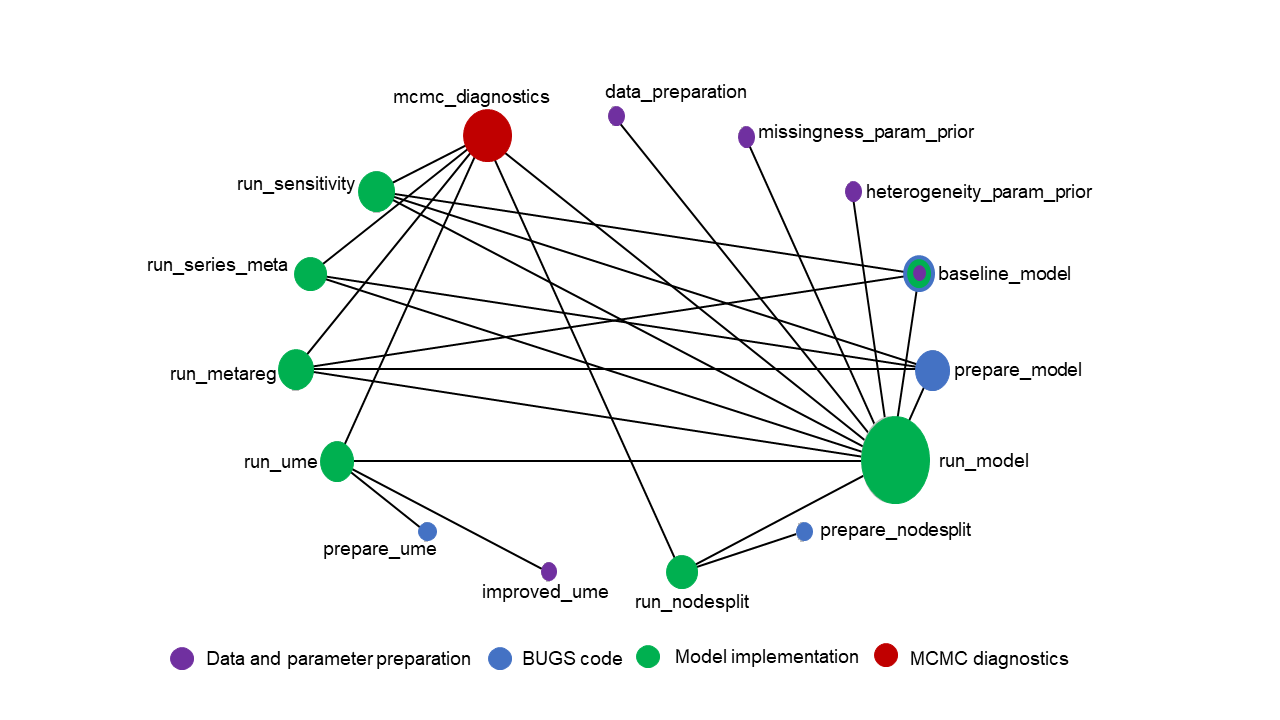
\includegraphics[width=1\linewidth,height=0.3\textheight]{network_models} \caption{Network of functions for data preparation and model implementation}\label{fig:network-models}
\end{figure}

\hypertarget{the-visualisation-toolkit}{%
\subsection{The visualisation toolkit}\label{the-visualisation-toolkit}}

Figure \ref{fig:network-visualisation} presents the network of visualisation-related
functions alongside \texttt{run\_model()} and several model-related functions. The
functions associated with summarising and presenting the results have a common
structure: \texttt{run\_model()} and the model-related function of interest are passed as
objects into the corresponding arguments. Hence, \texttt{run\_model()} comprises the backbone
of the network and forms the largest node (Figure \ref{fig:network-visualisation}).
The visualisation-related functions are distinguished into the \emph{stand-alone} and
the \emph{platform} functions. The stand-alone functions are immediately related to
generating the relevant graphs. For instance, \texttt{forestplot\_metareg()}, and \texttt{interval\_panel\_ume()}
constitute stand-alone functions and return only the intended graph using \texttt{run\_model()}
together with \texttt{run\_metareg()} and \texttt{run\_ume()}, respectively, as objects in their
arguments. Other stand-alone functions depend on a single function to operate;
for example, \texttt{rankosucra\_plot()} and \texttt{kld\_plot()} use only the \texttt{run\_model()} and
\texttt{robustness\_index()}, respectively, in their arguments. The platform functions
host the stand-alone functions and generate complementary tables and further graphs.
They are easy to spot in Figure \ref{fig:network-visualisation}, as they are named
after the related model, with the \emph{plot} affixed at the end: \texttt{nodesplit\_plot()},
\texttt{ume\_plot()}, \texttt{metareg\_plot()}, and \texttt{series\_meta\_plot()}. For instance,
\texttt{metareg\_plot()} calls \texttt{scatterplot\_sucra()} and \texttt{forestplot\_sucra()} to return
the corresponding intended graphs and prints tables in the console where the
effect estimates and predictions from NMA are juxtaposed with those from network
meta-regression. Every analysis has an individualised visualisation toolkit,
indicated by the functions sharing the same colour node (Figure \ref{fig:network-visualisation}).
Only network meta-regression (blue nodes) and conducting separate pairwise
meta-analyses (green nodes) share a few stand-alone functions with NMA (grey nodes),
namely, \texttt{league\_heatmap()} and \texttt{league\_heatmap\_pred()}.

\begin{figure}
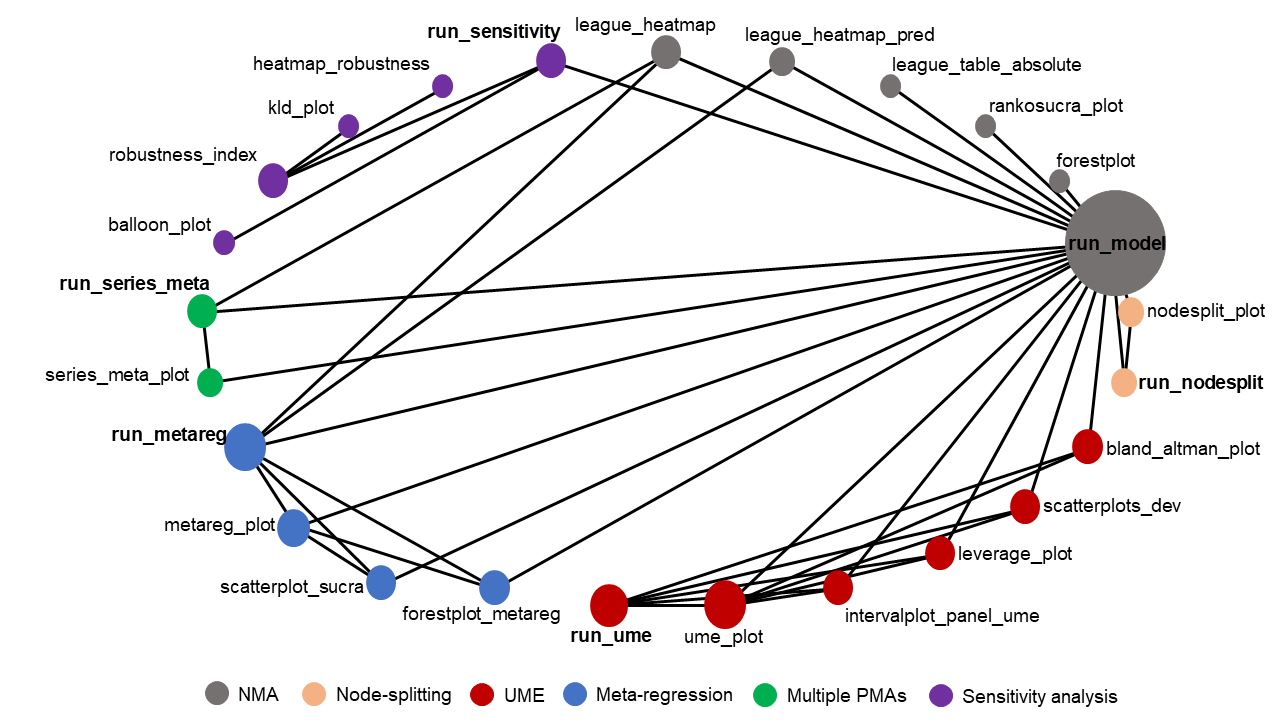
\includegraphics[width=1\linewidth,height=0.3\textheight]{network_visualisation} \caption{Network of functions for summarising and presenting the analysis results}\label{fig:network-visualisation}
\end{figure}

\hypertarget{a-gallery-of-tooltips-examples}{%
\section{A gallery of tooltips examples}\label{a-gallery-of-tooltips-examples}}

\hypertarget{summary}{%
\section{Summary}\label{summary}}

We have displayed various tooltips that are available in the package \pkg{ToOoOlTiPs}.

\hypertarget{references}{%
\section*{References}\label{references}}
\addcontentsline{toc}{section}{References}

\hypertarget{refs}{}
\begin{CSLReferences}{1}{0}
\leavevmode\vadjust pre{\hypertarget{ref-Akl2013}{}}%
Akl, Elie A, Bradley C Johnston, Pablo Alonso-Coello, Ignacio Neumann, Shanil Ebrahim, Matthias Briel, Deborah J Cook, and Gordon H Guyatt. 2013. {``Addressing Dichotomous Data for Participants Excluded from Trial Analysis: A Guide for Systematic Reviewers.''} \emph{PLoS One} 8 (2): e57132. \url{https://doi.org/10.1371/journal.pone.0057132}.

\leavevmode\vadjust pre{\hypertarget{ref-Bakbergenuly2019}{}}%
Bakbergenuly, Ilyas, David C Hoaglin, and Elena Kulinskaya. 2019. {``Pitfalls of Using the Risk Ratio in Meta-Analysis.''} \emph{Res Synth Methods} 10 (3): 398--419. \url{https://doi.org/10.1002/jrsm.1347}.

\leavevmode\vadjust pre{\hypertarget{ref-Bucher1997}{}}%
Bucher, H C, G H Guyatt, L E Griffith, and S D Walter. 1997. {``The Results of Direct and Indirect Treatment Comparisons in Meta-Analysis of Randomized Controlled Trials.''} \emph{J Clin Epidemiol} 50 (6): 683--91. \url{https://doi.org/10.1016/s0895-4356(97)00049-8}.

\leavevmode\vadjust pre{\hypertarget{ref-Caldwell2014}{}}%
Caldwell, Deborah M. 2014. {``An Overview of Conducting Systematic Reviews with Network Meta-Analysis.''} \emph{Syst Rev} 3: 109. \url{https://doi.org/10.1186/2046-4053-3-109}.

\leavevmode\vadjust pre{\hypertarget{ref-CRANTaskReview}{}}%
Dewey, Michael, and Wolfgang Viechtbauer. 2023. \emph{{CRAN Task View}: Meta-Analysis}. \url{https://CRAN.R-project.org/view=MetaAnalysis}.

\leavevmode\vadjust pre{\hypertarget{ref-Dias2016}{}}%
Dias, Sofia, and A E Ades. 2016. {``Absolute or Relative Effects? Arm-Based Synthesis of Trial Data.''} \emph{Res Synth Methods} 7 (1): 23--28. \url{https://doi.org/10.1002/jrsm.1184}.

\leavevmode\vadjust pre{\hypertarget{ref-Dias2013}{}}%
Dias, Sofia, Alexander J Sutton, A E Ades, and N J Welton. 2013. {``Evidence Synthesis for Decision Making 2: A Generalized Linear Modeling Framework for Pairwise and Network Meta-Analysis of Randomized Controlled Trials.''} \emph{Med Decis Making} 33 (5): 607--17.

\leavevmode\vadjust pre{\hypertarget{ref-GetRealNMA}{}}%
Efthimiou, Orestis, Thomas P. A. Debray, Gert van Valkenhoef, Sven Trelle, Klea Panayidou, Karel G. M. Moons, Johannes B. Reitsma, Aijing Shang, Georgia Salanti, and GetReal Methods Review Group. 2016. {``GetReal in Network Meta-Analysis: A Review of the Methodology.''} \emph{Res Synth Methods} 7 (3): 236--63. \url{https://doi.org/10.1002/jrsm.1195}.

\leavevmode\vadjust pre{\hypertarget{ref-Friedrich2008}{}}%
Friedrich, Jan O, Neill K J Adhikari, and Joseph Beyene. 2008. {``The Ratio of Means Method as an Alternative to Mean Differences for Analyzing Continuous Outcome Variables in Meta-Analysis: A Simulation Study.''} \emph{BMC Med Res Methodol} 8: 32. \url{https://doi.org/10.1186/1471-2288-8-32}.

\leavevmode\vadjust pre{\hypertarget{ref-Higgins2008}{}}%
Higgins, Julian P T, Ian R White, and Angela M Wood. 2008. {``Imputation Methods for Missing Outcome Data in Meta-Analysis of Clinical Trials.''} \emph{Clin Trials} 5 (3): 225--39. \url{https://doi.org/10.1177/1740774508091600}.

\leavevmode\vadjust pre{\hypertarget{ref-Higgins1996}{}}%
Higgins, Julian P T, and Anne Whitehead. 1996. {``Borrowing Strength from External Trials in a Meta-Analysis.''} \emph{Stat Med} 15 (24): 2733--49.

\leavevmode\vadjust pre{\hypertarget{ref-Lee2022}{}}%
Lee, Andrew. 2022. {``The Development of Network Meta-Analysis.''} \emph{J R Soc Med} 115 (8): 313--21. \url{https://doi.org/10.1177/01410768221113196}.

\leavevmode\vadjust pre{\hypertarget{ref-pcnetmeta}{}}%
Lin, Lifeng, Jing Zhang, James S. Hodges, and Haitao Chu. 2017. {``Performing Arm-Based Network Meta-Analysis in {R} with the {pcnetmeta} Package.''} \emph{Journal of Statistical Software} 80 (5): 1--25. \url{https://doi.org/10.18637/jss.v080.i05}.

\leavevmode\vadjust pre{\hypertarget{ref-Little1993}{}}%
Little, RJA. 1993. {``Pattern-Mixture Models Formultivariate Incomplete Data.''} \emph{J Am Stat Assoc} 88 (421): 125--34. \url{https://doi.org/doi.org/10.2307/2290705}.

\leavevmode\vadjust pre{\hypertarget{ref-Little1995}{}}%
---------. 1995. {``Modeling the Drop-Out Mechanism in Repeated-Measures Studies.''} \emph{J Am Stat Assoc} 90 (431): 1112--21. \url{https://doi.org/10.2307/2291350}.

\leavevmode\vadjust pre{\hypertarget{ref-Lunn2009}{}}%
Lunn, David, David Spiegelhalter, Andrew Thomas, and Nicky Best. 2009. {``The BUGS Project: Evolution, Critique and Future Directions.''} \emph{Stat Med} 28 (25): 3049--67. \url{https://doi.org/10.1002/sim.3680}.

\leavevmode\vadjust pre{\hypertarget{ref-Magder2003}{}}%
Magder, Laurence S. 2003. {``Simple Approaches to Assess the Possible Impact of Missing Outcome Information on Estimates of Risk Ratios, Odds Ratios, and Risk Differences.''} \emph{Control Clin Trials} 24 (4): 411--21. \url{https://doi.org/10.1016/s0197-2456(03)00021-7}.

\leavevmode\vadjust pre{\hypertarget{ref-Mavridis2015}{}}%
Mavridis, Dimitris, Ian R White, Julian P T Higgins, Andrea Cipriani, and Georgia Salanti. 2015. {``Allowing for Uncertainty Due to Missing Continuous Outcome Data in Pairwise and Network Meta-Analysis.''} \emph{Stat Med} 34 (5): 721--41. \url{https://doi.org/10.1002/sim.6365}.

\leavevmode\vadjust pre{\hypertarget{ref-Carpenter2007}{}}%
\emph{Missing Data in Randomised Controlled Trials: A Practical Guide.} 2007. Health Technology Assessment Methodology Programme: Birmingham. \url{https://researchonline.lshtm.ac.uk/id/eprint/4018500}.

\leavevmode\vadjust pre{\hypertarget{ref-Nikolakopoulou2014}{}}%
Nikolakopoulou, Adriani, Anna Chaimani, Areti Angeliki Veroniki, Haris S Vasiliadis, Christopher H Schmid, and Georgia Salanti. 2014. {``Characteristics of Networks of Interventions: A Description of a Database of 186 Published Networks.''} \emph{PLoS One} 9 (1): e86754. \url{https://doi.org/10.1371/journal.pone.0086754}.

\leavevmode\vadjust pre{\hypertarget{ref-Petropoulou2017}{}}%
Petropoulou, Maria, Adriani Nikolakopoulou, Areti-Angeliki Veroniki, Patricia Rios, Afshin Vafaei, Wasifa Zarin, Myrsini Giannatsi, et al. 2017. {``Bibliographic Study Showed Improving Statistical Methodology of Network Meta-Analyses Published Between 1999 and 2015.''} \emph{J Clin Epidemiol} 82: 20--28. \url{https://doi.org/10.1016/j.jclinepi.2016.11.002}.

\leavevmode\vadjust pre{\hypertarget{ref-Plummer2003}{}}%
Plummer, Martyn. 2003. \emph{JAGS: A Program for Analysis of Bayesian Graphical Models Using Gibbs Sampling}. Edited by Kurt Hornik, Friedrich Leisch, and Achim Zeileis. Technische Universität Wien, Vienna, Austria. \url{https://www.R-project.org/conferences/DSC-2003/Proceedings/Plummer.pdf}.

\leavevmode\vadjust pre{\hypertarget{ref-R2023}{}}%
R Core Team. 2023. {``{R: A Language and Environment for Statistical Computing}. Foundation for Statistical Computing, Vienna, Austria.''} \url{https://www.R-project.org/}.

\leavevmode\vadjust pre{\hypertarget{ref-EvidenceBasedMedicine}{}}%
Sackett, David L, William M Rosenberg, J A Gray, R B Haynes, and W S Richardson. 1996. {``Evidence Based Medicine: What It Is and What It Isn't.''} \emph{BMJ} 312 (7023): 71--72. \url{https://doi.org/10.1136/bmj.312.7023.71}.

\leavevmode\vadjust pre{\hypertarget{ref-Salanti2012}{}}%
Salanti, Georgia. 2012. {``Indirect and Mixed-Treatment Comparison, Network, or Multiple-Treatments Meta-Analysis: Many Names, Many Benefits, Many Concerns for the Next Generation Evidence Synthesis Tool.''} \emph{Res Synth Methods} 3 (2): 80--97. \url{https://doi.org/10.1002/jrsm.1037}.

\leavevmode\vadjust pre{\hypertarget{ref-Salanti2022}{}}%
Salanti, Georgia, Adriani Nikolakopoulou, Orestis Efthimiou, Dimitris Mavridis, Matthias Egger, and Ian R White. 2022. {``Introducing the Treatment Hierarchy Question in Network Meta-Analysis.''} \emph{Am J Epidemiol} 191 (5): 930--38. \url{https://doi.org/10.1093/aje/kwab278}.

\leavevmode\vadjust pre{\hypertarget{ref-SAS2020}{}}%
SAS Institute. 2020. {``{The SAS System for Windows}. Release 9.4. Cary, NC: SAS Inst.''} \url{https://www.sas.com}.

\leavevmode\vadjust pre{\hypertarget{ref-bnma}{}}%
Seo, Michael, and Christopher Schmid. 2022. \emph{Bnma: Bayesian Network Meta-Analysis Using 'JAGS'}. \url{https://CRAN.R-project.org/package=bnma}.

\leavevmode\vadjust pre{\hypertarget{ref-Spineli2019}{}}%
Spineli, Loukia M. 2019. {``An Empirical Comparison of Bayesian Modelling Strategies for Missing Binary Outcome Data in Network Meta-Analysis.''} \emph{BMC Med Res Methodol} 19 (1): 86. \url{https://doi.org/10.1186/s12874-019-0731-y}.

\leavevmode\vadjust pre{\hypertarget{ref-rnmamod}{}}%
---------. 2022. \emph{Rnmamod: Bayesian Network Meta-Analysis with Missing Participants}. \url{https://CRAN.R-project.org/package=rnmamod}.

\leavevmode\vadjust pre{\hypertarget{ref-Stata}{}}%
StataCorp. 2021. {``{Stata Statistical Software: Release 17}. College Station, TX: StataCorp LLC.''} \url{http://www.stata.com}.

\leavevmode\vadjust pre{\hypertarget{ref-R2jags}{}}%
Su, Yu-Sung, and Masanao Yajima. 2021. \emph{R2jags: Using r to Run 'JAGS'}. \url{https://CRAN.R-project.org/package=R2jags}.

\leavevmode\vadjust pre{\hypertarget{ref-Sutton2001}{}}%
Sutton, Alex J, and Keith R Abrams. 2001. {``Bayesian Methods in Meta-Analysis and Evidence Synthesis.''} \emph{Stat Methods Med Res} 10 (4): 277--303. \url{https://doi.org/10.1177/096228020101000404}.

\leavevmode\vadjust pre{\hypertarget{ref-NationalResearchCouncil}{}}%
\emph{The Prevention and Treatment of Missing Data in Clinical Trials Panel on Handling Missing Data in Clinical Trials.} 2010. Division of Behavioral; Social Sciences; Education, Washington, DC: The National Academies Press. \href{https://www.nap.edu}{www.nap.edu}.

\leavevmode\vadjust pre{\hypertarget{ref-Turner2015}{}}%
Turner, N. L., S. Dias, A. E. Ades, and N. J. Welton. 2015. {``A Bayesian Framework to Account for Uncertainty Due to Missing Binary Outcome Data in Pairwise Meta-Analysis.''} \emph{Stat Med} 34 (12): 2062--80. \url{https://doi.org/10.1002/sim.6475}.

\leavevmode\vadjust pre{\hypertarget{ref-gemtc}{}}%
van Valkenhoef, Gert, and Joel Kuiper. 2021. \emph{Gemtc: Network Meta-Analysis Using Bayesian Methods}. \url{https://CRAN.R-project.org/package=gemtc}.

\leavevmode\vadjust pre{\hypertarget{ref-White2007}{}}%
White, Ian R, James Carpenter, Stephen Evans, and Sara Schroter. 2007. {``Eliciting and Using Expert Opinions about Dropout Bias in Randomized Controlled Trials.''} \emph{Clin Trials} 4 (2): 125--39. \url{https://doi.org/10.1177/1740774507077849}.

\leavevmode\vadjust pre{\hypertarget{ref-White2008}{}}%
White, Ian R, Julian P T Higgins, and Angela M Wood. 2008. {``Allowing for Uncertainty Due to Missing Data in Meta-Analysis---Part 1: Two-Stage Methods.''} \emph{Stat Med} 27 (5): 711--27. \url{https://doi.org/10.1002/sim.3008}.

\leavevmode\vadjust pre{\hypertarget{ref-ggplot2}{}}%
Wickham, Hadley. 2016. \emph{Ggplot2: Elegant Graphics for Data Analysis}. Springer-Verlag New York. \url{https://ggplot2.tidyverse.org}.

\end{CSLReferences}

\bibliography{RJreferences.bib}

\address{%
Loukia M. Spineli\\
Midwifery Research and Education Unit\\%
Hannover Medical School\\ Carl-Neuber-Strasse 1, 30625, Hannover, Germany\\
%
\url{https://www.github.com/LoukiaSpin}\\%
\textit{ORCiD: \href{https://orcid.org/0000-0001-9515-582X}{0000-0001-9515-582X}}\\%
\href{mailto:Spineli.Loukia@mh-hannover.de}{\nolinkurl{Spineli.Loukia@mh-hannover.de}}%
}

\address{%
Chrysostomos Kalyvas\\
Biostatistics and Research Decision Sciences\\%
MSD Europe Inc., Brussels, Belgium\\
%
\url{https://www.github.com/ckalyvas}\\%
\textit{ORCiD: \href{https://orcid.org/0000-0003-0606-4518}{0000-0003-0606-4518}}\\%
\href{mailto:chrysostomos.kalyvas@merck.com}{\nolinkurl{chrysostomos.kalyvas@merck.com}}%
}

\address{%
Katerina Papadimitropoulou\\
Health Economics and Market Access\\%
Amaris Consulting, Lyon, France\\
%
\url{https://www.github.com/Katerina-Pap}\\%
\textit{ORCiD: \href{https://orcid.org/0000-0002-5732-4044}{0000-0002-5732-4044}}\\%
\href{mailto:katerina.papadimitropoulou@gmail.com}{\nolinkurl{katerina.papadimitropoulou@gmail.com}}%
}
